\section{Triangle inequalities}

\begin{theorem*}
  Let $a,b \in \R$. Then
  \begin{align*}
    ||a| - |b|| \leq |a + b| \leq |a| + |b|.
  \end{align*}
\end{theorem*}

\section{Completing the square and the quadratic formula}

The quadratic equation $ax^2 + bx + c = 0$ can be solved as follows:
\begin{align*}
  ax^2 + bx + c                             &= 0\\
  \(\sqrt{a}x + \frac{b}{2\sqrt{a}}\)^2 - \frac{b^2}{4a} + c &= 0\\
  \sqrt{a}x &= \sqrt{\frac{b^2 - 4ac}{4a}} - \frac{b}{2\sqrt{a}}\\
  x &= \frac{-b \pm \sqrt{b^2 - 4ac}}{2a}.
\end{align*}

\section{Partial fractions}

\begin{align*}
  \frac{1}{xy} = \frac{A}{x} + \frac{B}{y}
\end{align*}

\section{Even and odd functions}

\begin{definition*}
  A function (over an additive group?) is even if and only if $f(-x) = f(x)$ for all $x$.

  A function (over an additive group?) is odd if and only if $f(-x) = -f(x)$ for all $x$.
\end{definition*}

Functions can be neither even nor odd.

\begin{claim*}
  A polynomial $p(x)$ is even if an only if it has only even powers of $x$.

  A polynomial $p(x)$ is odd if an only if it has only odd powers of $x$.
\end{claim*}

\section{$\sqrt{2}$ is irrational}
\begin{claim*}
  $\sqrt{2}$ is irrational.
\end{claim*}

\begin{proof}
  Suppose $\sqrt{2} \in \Q$. Then $\sqrt{2}$ can be written as $\frac{a}{b}$ where $a, b \in \Z$
  have no common factor (aka coprime, aka mutually prime).

  Then $2 = \frac{a^2}{b^2}$, so $a^2$ is even.

  Therefore $a$ is even.

  Let $a = 2c$. Then $b^2 = \frac{4c^2}{2} = 2c^2$, so $b^2$ is even.

  Therefeore both $a$ and $b$ are even, which is a contradiction.

  Therefore $\sqrt{2} \notin \Q$.
\end{proof}


\section{Misc}
\begin{mdframed}
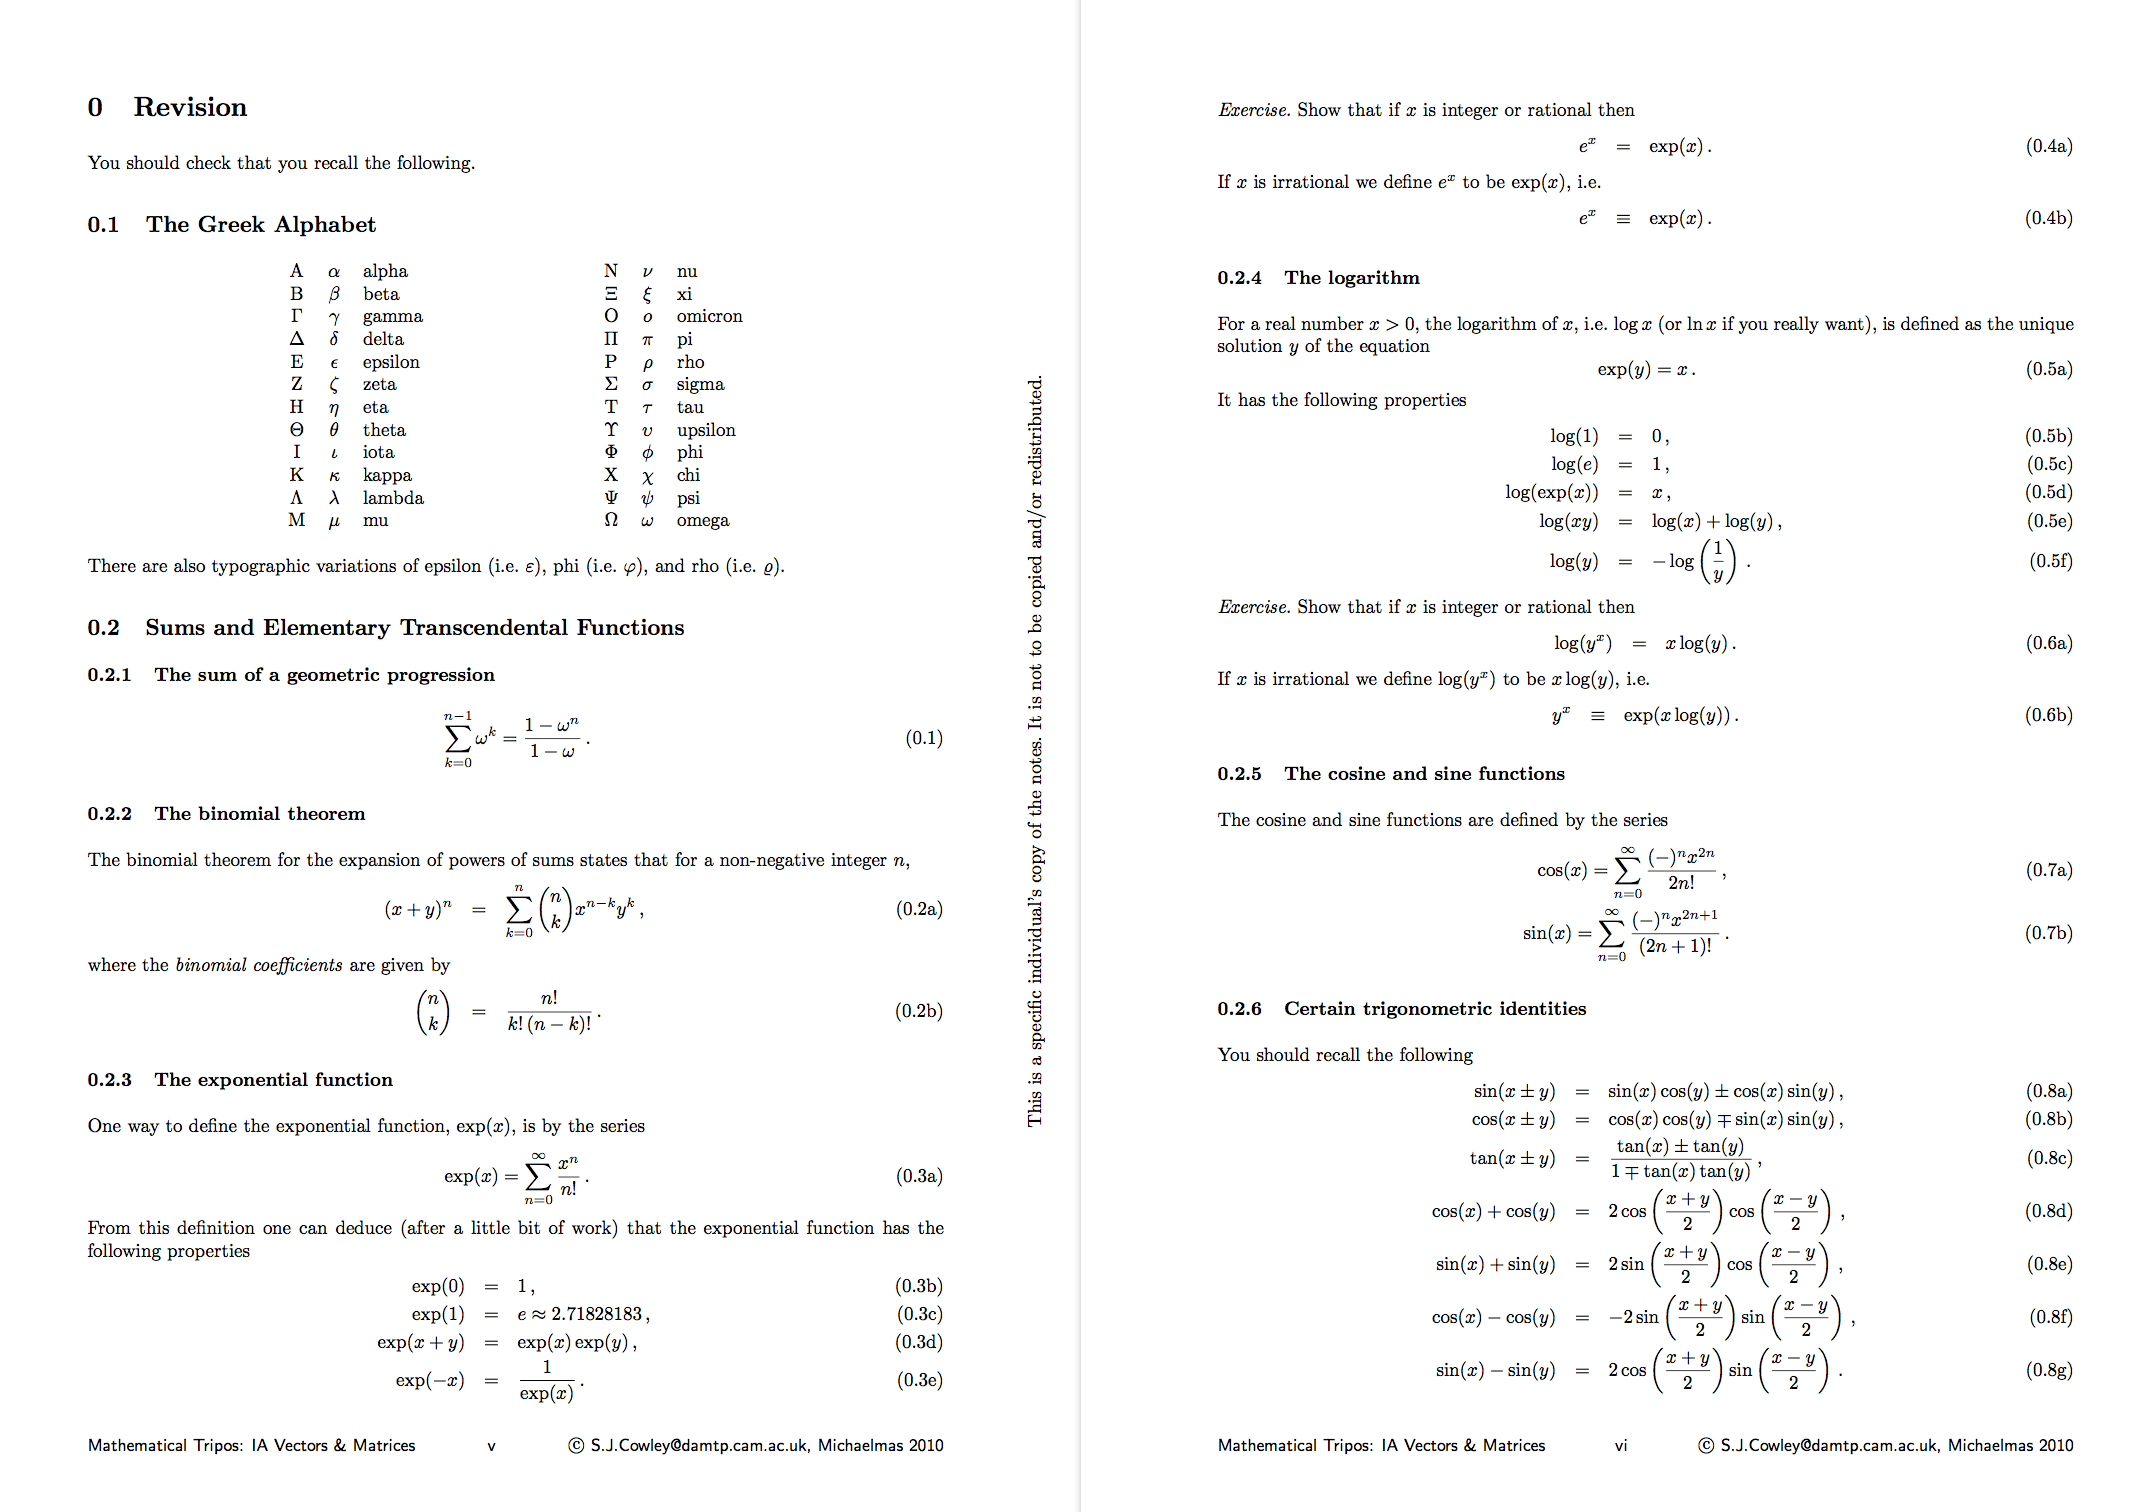
\includegraphics[width=400pt]{img/misc--cambridge-1a-vectors-and-matrices-revision-1.png}
\end{mdframed}
\begin{mdframed}
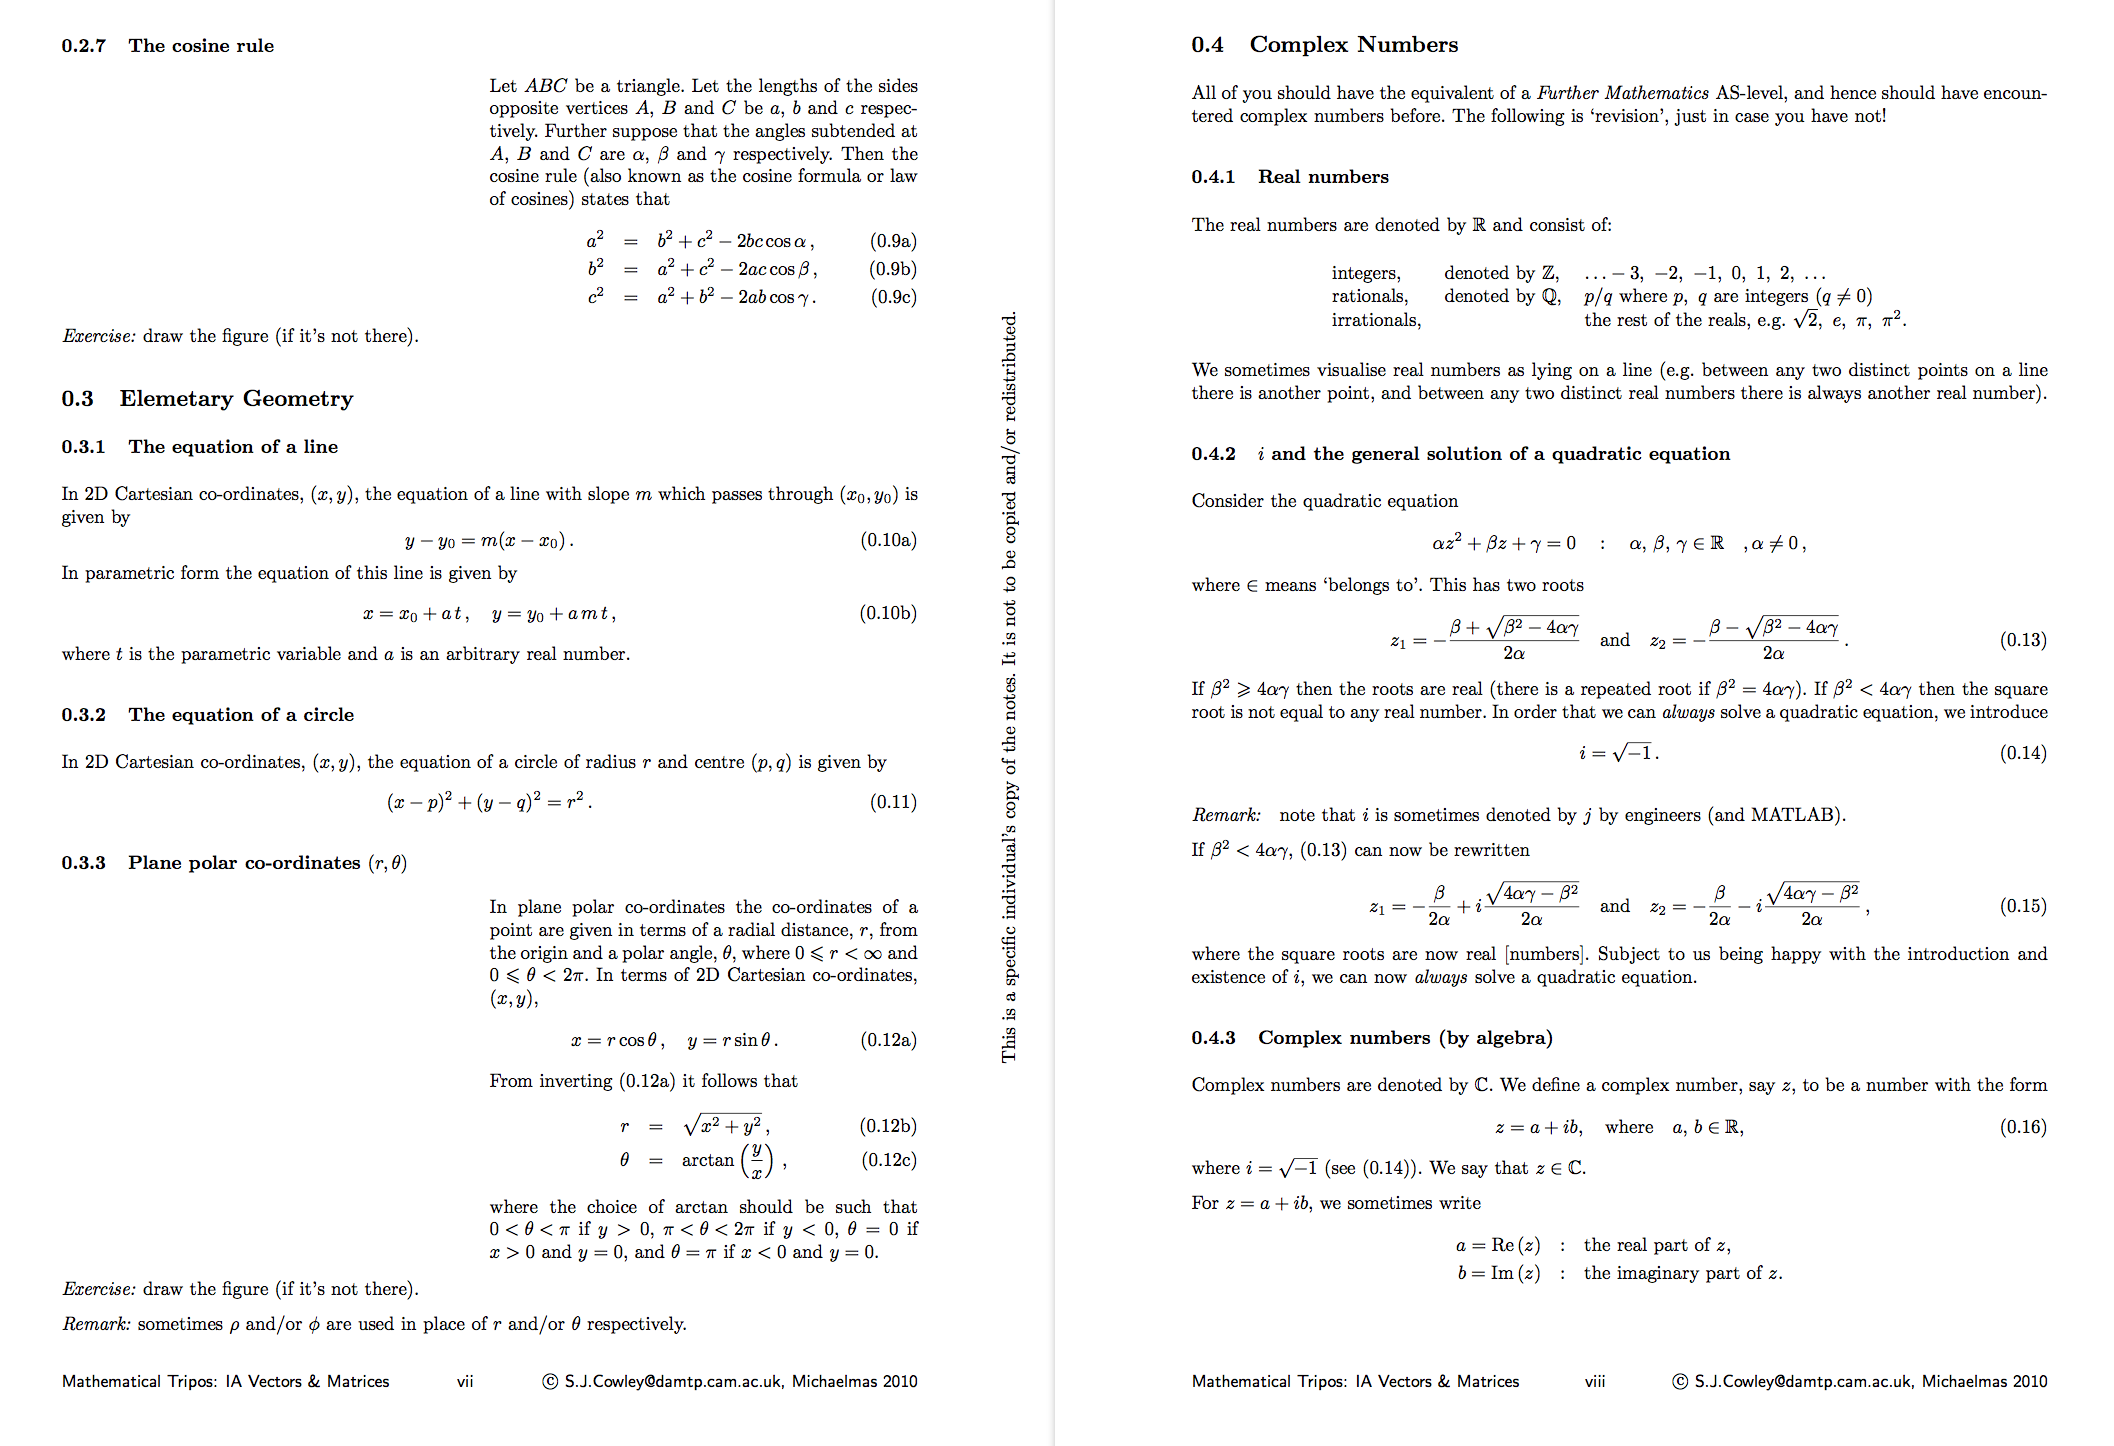
\includegraphics[width=400pt]{img/misc--cambridge-1a-vectors-and-matrices-revision-2.png}
\end{mdframed}
\begin{mdframed}
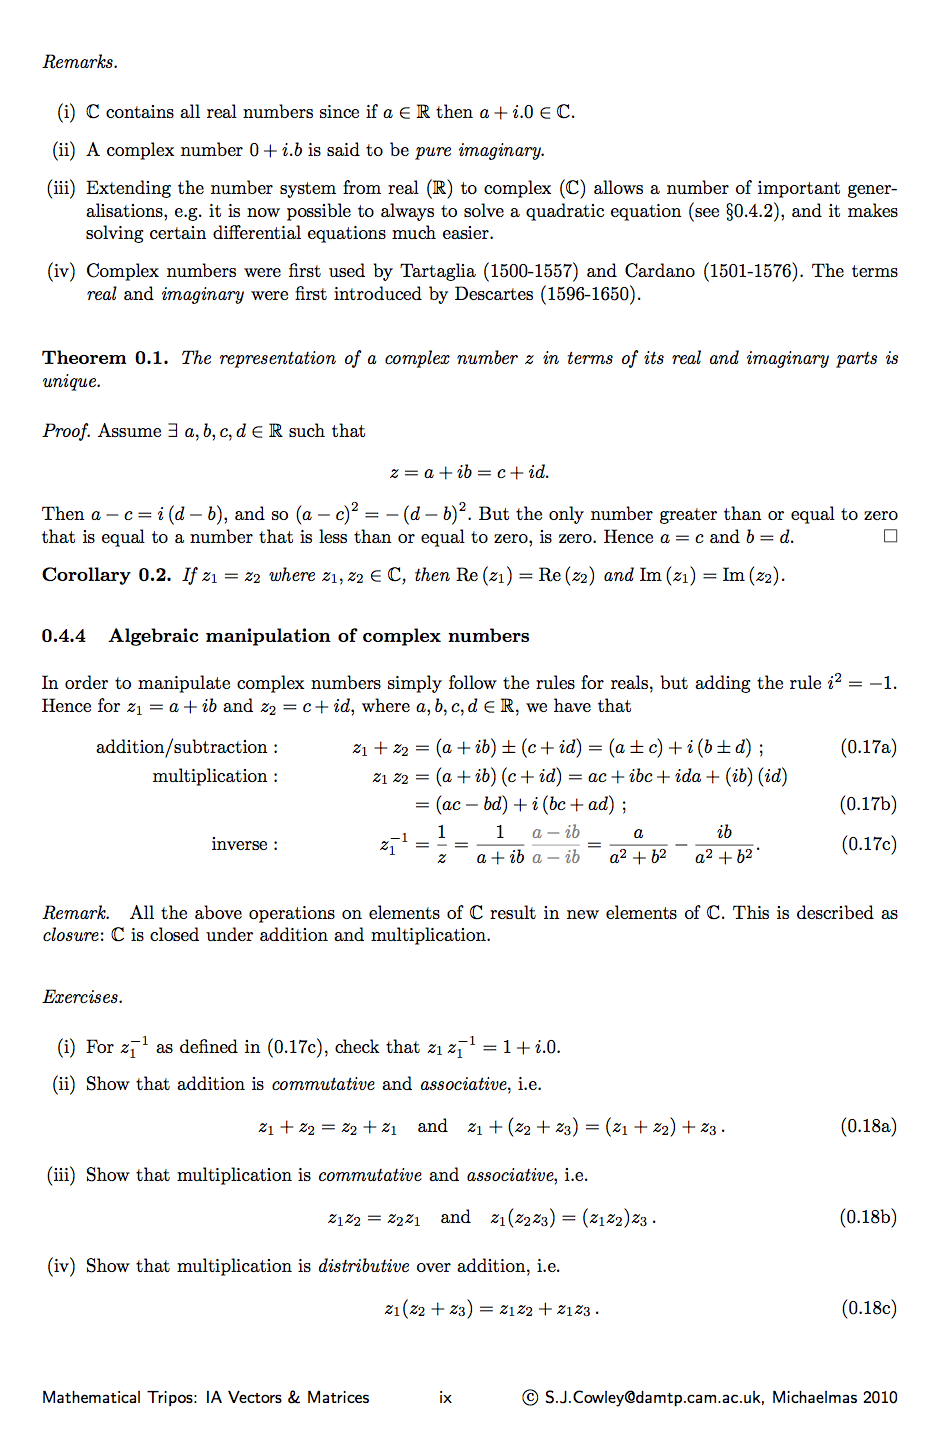
\includegraphics[width=400pt]{img/misc--cambridge-1a-vectors-and-matrices-revision-3.png}
\end{mdframed}